\documentclass[a4paper,12pt]{article} % тип документа
\usepackage[margin=1in]{geometry} % Поля

%  Русский язык
\usepackage[warn]{mathtext}
\usepackage[T2A]{fontenc}			% кодировка
\usepackage[utf8]{inputenc}			% кодировка исходного текста
\usepackage[english,russian]{babel}	% локализация и переносы
% Математика
\usepackage{amsmath,amsfonts,amssymb,amsthm,mathtools} 
\usepackage{wasysym}
%%%
\usepackage{graphicx}

\usepackage{tabularx}

\usepackage{gensymb} % знак градуса
\usepackage{enumitem} % изменить список enumerate
\usepackage{placeins} % \FloatBarrier

\renewcommand{\thesection}{\Roman{section}} 
\renewcommand{\thesubsection}{\roman{subsection}}
\renewcommand{\thesubsubsection}{\roman{subsection}.\roman{subsubsection}}


\begin{document}

\newcolumntype{Y}{>{\centering\arraybackslash}X} %new tabularx


%титул

\begin{center}
{\LARGE Московский Физико-Технический Институт}
\\
{\large Физтех-школа электроники, фотоники и молекулярной физики }
\\
\vspace{8cm}
{\LARGE Отчёт по лабораторной работе:}
\\
{\Huge Конвективная диффузия в молекулярно- электронных преобразователях} 
\\
\vspace{5cm}
\raggedright 
\hspace{7cm}{\large Выполнили студенты группы Б04-005}\\
\hspace{7cm}{\large Карташов Констанин}\\
\hspace{7cm}{\large Давыдов Владислав}

\vspace{\fill}
\center
{\large Долгопрудный 2022}

\end{center}

\newpage


\section{Анотация}

\paragraph{Цель работы:} 
Изучение работы газоразрядного стабилизатора напряжения. Снятие кривой Пашена и 
\paragraph{Оборудование:}
\begin{itemize}
\renewcommand{\labelitemi}{$\triangleright$}
\itemsep0em
\item Вакуумная установка,
\item Газоразрядная трубка,
\item Лабораторный блок питания.
\end{itemize}



\medskip\hrule\medskip

\section{Экспериментальная часть}

\subsection{Кривая Пашена}

\paragraph{} При постоянном токе на стабилитроне, измерим зависимость напряжения от давления газов (\ref{fig:pash}). По измеренным данным построим кривуцю пашена (\ref{fig:pash}). Видим, что минимум кривой приходится на $u = 0.68$ Кв при $p= 0.168$ торр.

\begin{table}[h]
\centering
\begin{tabular}{|l|l|l|l|l|l|l|l|}
\hline
$P$, торр & 1.400 & 0.827 & 0.400 & 0.240 & 0.219 & 0.200 & 0.182 \\ \hline
$U$, кВ   & 0.8   & 0.72  & 0.69  & 0.7   & 0.69  & 0.69  & 0.68  \\ \hline
$P$, торр & 0.164 & 0.144 & 0.123 & 0.101 & 0.078 & 0.051 & --    \\ \hline
$U$, кВ   & 0.69  & 0.69  & 0.72  & 0.77  & 1.08  & 1.93  & --    \\ \hline
\end{tabular}
\caption{}
\label{tab:pash}
\end{table}

\begin{figure}[h]
\centering
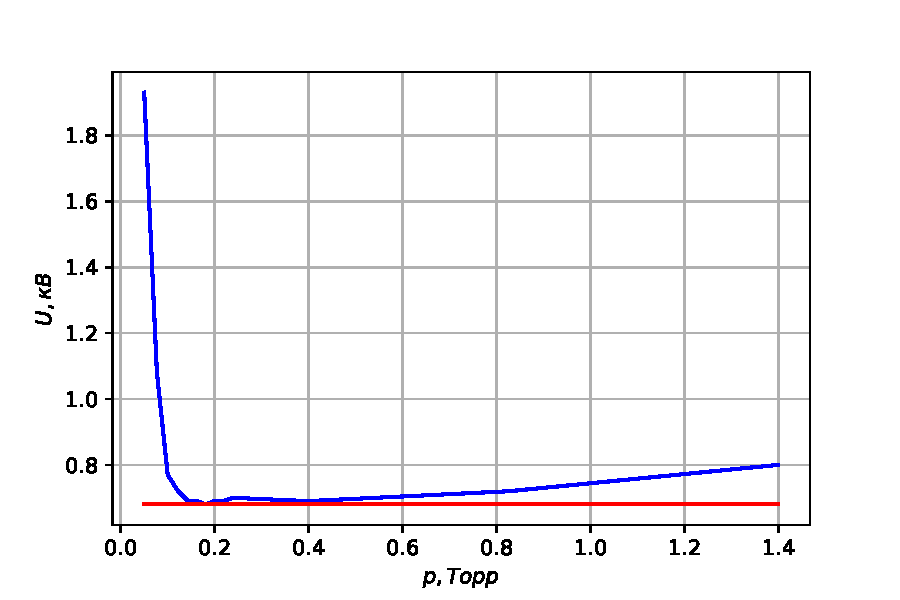
\includegraphics[width=\textwidth]{un-pashe.pdf}
\caption{Кривая Пашена}
\label{fig:pash}
\end{figure}


\subsection{ВАХ стабилитрона}

\paragraph{} Теперь при постоянном давлении $p \approx 0.2$ торр будем менять ток. Снимем вольт-амперную характеристику (\ref{tab:vac}). Построим график ВАХ (\ref{fig:afc}). Видим, что график соответствует 3-му участку ВАХ газоразрядного диода.

\begin{table}[h]
\centering
\begin{tabular}{|l|l|l|l|l|l|}
\hline
$U$, кВ           & 0.69 & 0.7  & 0.72 & 0.73 & 0.74 \\ \hline
$I, \; 10^{-4}$ А & 19   & 17   & 15   & 13   & 11   \\ \hline
$U$, кВ           & 0.75 & 0.75 & 0.76 & 0.8  & 0.78 \\ \hline
$I, \; 10^{-4}$ А & 9    & 7    & 5    & 3    & 1    \\ \hline
\end{tabular}
\caption{Вольт-амперная характеристика стабиловольта}
\label{tab:vac}
\end{table}

\begin{figure}[h]
\centering
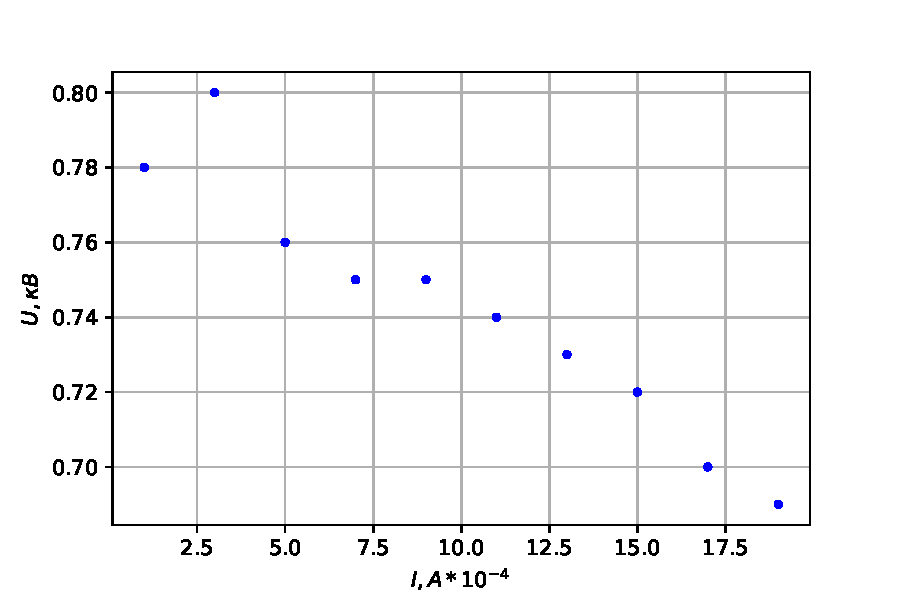
\includegraphics[width=\textwidth]{vah.pdf}
\caption{График вольт-амперной характеристики стабиловольта}
\label{fig:afc}
\end{figure}




\medskip\hrule\medskip


\end{document}
